\section{Neural Networks 101}
\label{sec:neural_networks_101}
% PROMPT: Showcase a minimal neural network from scratch

\begin{figure}[h]
\centering
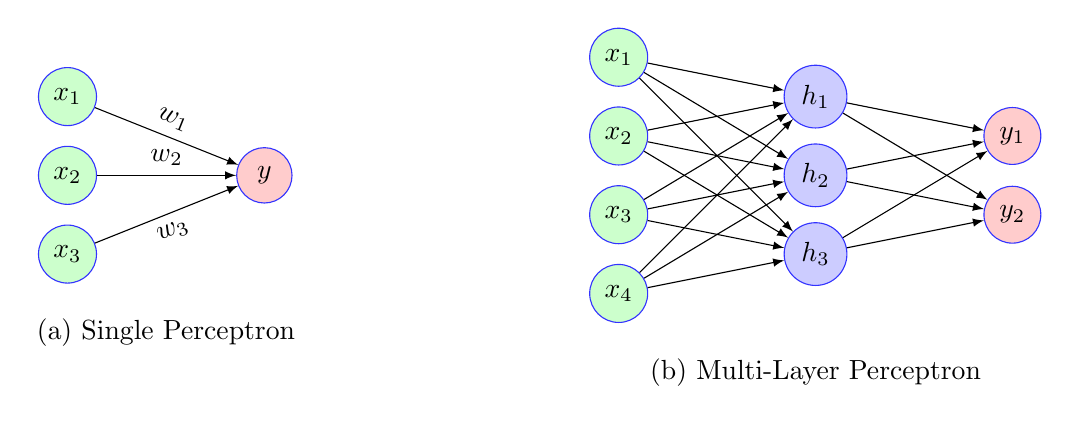
\begin{tikzpicture}[
    neuron/.style={circle, draw=blue!80, fill=blue!20, minimum size=20pt},
    input/.style={neuron, fill=green!20},
    output/.style={neuron, fill=red!20},
    >=latex
]
% Single Perceptron
\begin{scope}[xshift=-3cm]
    % Inputs
    \node[input] (x1) at (0,1) {$x_1$};
    \node[input] (x2) at (0,0) {$x_2$};
    \node[input] (x3) at (0,-1) {$x_3$};
    
    % Output neuron
    \node[output] (y) at (2.5,0) {$y$};
    
    % Connections
    \draw[->] (x1) -- node[above, sloped] {$w_1$} (y);
    \draw[->] (x2) -- node[above] {$w_2$} (y);
    \draw[->] (x3) -- node[below, sloped] {$w_3$} (y);
    
    % Title
    \node[align=center] at (1.25,-2) {(a) Single Perceptron};
\end{scope}

% Multi-Layer Perceptron
\begin{scope}[xshift=4cm]
    % Input layer
    \node[input] (i1) at (0,1.5) {$x_1$};
    \node[input] (i2) at (0,0.5) {$x_2$};
    \node[input] (i3) at (0,-0.5) {$x_3$};
    \node[input] (i4) at (0,-1.5) {$x_4$};
    
    % Hidden layer
    \node[neuron] (h1) at (2.5,1) {$h_1$};
    \node[neuron] (h2) at (2.5,0) {$h_2$};
    \node[neuron] (h3) at (2.5,-1) {$h_3$};
    
    % Output layer
    \node[output] (o1) at (5,0.5) {$y_1$};
    \node[output] (o2) at (5,-0.5) {$y_2$};
    
    % Connections for input to hidden layer
    \foreach \i in {1,2,3,4}
        \foreach \j in {1,2,3}
            \draw[->] (i\i) -- (h\j);
    
    % Connections for hidden to output layer
    \foreach \i in {1,2,3}
        \foreach \j in {1,2}
            \draw[->] (h\i) -- (o\j);
    
    % Title
    \node[align=center] at (2.5,-2.5) {(b) Multi-Layer Perceptron};
\end{scope}

\end{tikzpicture}
\caption{Neural Network Architectures: (a) Single perceptron computing $y = \sigma(\sum_{i} w_i x_i + b)$, where $\sigma$ is an activation function. 
(b) Multi-layer perceptron computing hidden layer $h_j = \sigma(\sum_{i} w^{(1)}_{ij} x_i + b^{(1)}_j)$ followed by outputs 
$y_k = \sigma(\sum_{j} w^{(2)}_{jk} h_j + b^{(2)}_k)$. This architecture enables learning complex non-linear mappings through multiple layers of transformation.}
\label{fig:neural_architectures}
\end{figure}

\noindent
Neural networks have revolutionized modern machine learning by learning \emph{non-linear} mappings from input features to output predictions without the need for manually engineered features. In the context of language modeling, neural networks are particularly powerful because they can encode and combine linguistic features in high-dimensional spaces, capturing nuances that simpler statistical models may overlook.

\subsection{Perceptrons and Multi-Layer Perceptrons (MLPs)}
\noindent
The \textbf{perceptron}, introduced by Frank Rosenblatt in the late 1950s, is one of the earliest forms of a trainable neural network. It models a single neuron with:
\begin{enumerate}
    \item A set of input weights.
    \item A linear combination of inputs and weights.
    \item A non-linear activation function (e.g., step function).
\end{enumerate}
While a single perceptron can only represent linear decision boundaries, stacking multiple perceptrons in layers (known as a \textbf{Multi-Layer Perceptron}, or MLP) allows for the modeling of highly complex, non-linear relationships.

\begin{itemize}
    \item \textbf{Input Layer.} Receives the raw features, such as token embeddings in NLP.
    \item \textbf{Hidden Layers.} Non-linear transformations are applied in each layer. Common activation functions include $\text{ReLU}, \tanh, \text{sigmoid}$.
    \item \textbf{Output Layer.} Produces the final prediction, such as a probability distribution over the next token for language modeling.
\end{itemize}

\subsection{Forward and Backpropagation}
\noindent
Learning in neural networks typically involves two main steps:
\begin{itemize}
    \item \textbf{Forward Propagation.} The input $\mathbf{x}$ is propagated through each layer of the network to compute an output $\hat{\mathbf{y}}$. Mathematically, for layer $l$ with weights $\mathbf{W}^{(l)}$ and bias $\mathbf{b}^{(l)}$,
    \begin{equation}\label{eq:forward_prop}
        \mathbf{z}^{(l)} = \mathbf{W}^{(l)} \mathbf{h}^{(l-1)} + \mathbf{b}^{(l)}, \quad \mathbf{h}^{(l)} = \sigma(\mathbf{z}^{(l)})
    \end{equation}
    where $\sigma(\cdot)$ is a non-linear activation function, and $\mathbf{h}^{(0)} \equiv \mathbf{x}$ is the input vector.

    \item \textbf{Backward Propagation (Backprop).} Once a loss function $\mathcal{L}(\hat{\mathbf{y}}, \mathbf{y})$ is computed—where $\mathbf{y}$ is the ground-truth label—the gradient of $\mathcal{L}$ w.r.t. each parameter in the network is calculated using the chain rule. Parameters are updated via an optimization algorithm (e.g., \textit{Stochastic Gradient Descent}, \textit{Adam}), moving them in the direction that reduces the loss.
\end{itemize}

\noindent
This loop of forward and backward propagation, repeated over multiple \emph{epochs} of training data, enables a neural network to \emph{learn} complex transformations—an essential capability for tasks like language modeling.

\subsection{Activation Functions}
\noindent
Activation functions impart non-linearity, allowing neural networks to model non-trivial functions.  See Figure \ref{fig:activation_functions} for a comparison of common activation functions.

\begin{figure}[h]
\centering
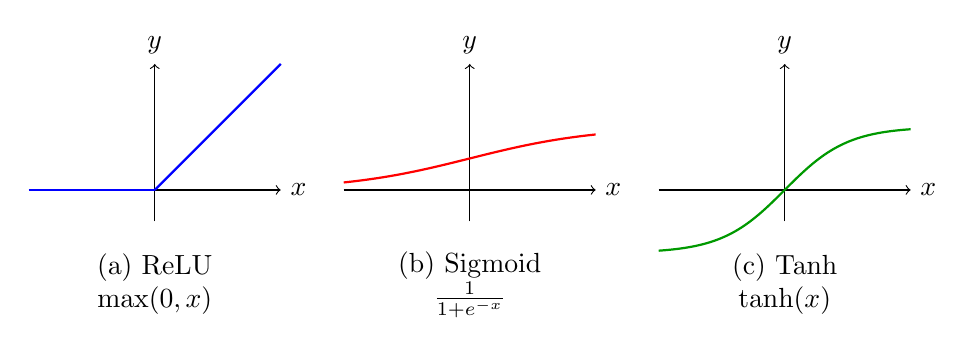
\begin{tikzpicture}[
    declare function={
        relu(\x) = max(0,\x);
        sigmoid(\x) = 1/(1 + exp(-\x));
        tanhy(\x) = (exp(\x) - exp(-\x))/(exp(\x) + exp(-\x));
    },
    scale=0.8
]
% Grid and axes for ReLU
\begin{scope}[xshift=-5cm]
    \draw[->] (-2,0) -- (2,0) node[right] {$x$};
    \draw[->] (0,-0.5) -- (0,2) node[above] {$y$};
    \draw[thick, blue] (-2,0) -- (0,0);
    \draw[thick, blue] (0,0) -- (2,2);
    \node[align=center] at (0,-1.5) {(a) ReLU\\$\max(0,x)$};
\end{scope}

% Grid and axes for Sigmoid
\begin{scope}[xshift=0cm]
    \draw[->] (-2,0) -- (2,0) node[right] {$x$};
    \draw[->] (0,-0.5) -- (0,2) node[above] {$y$};
    \draw[thick, red, domain=-2:2, samples=100] 
        plot (\x,{sigmoid(\x)});
    \node[align=center] at (0,-1.5) {(b) Sigmoid\\$\frac{1}{1+e^{-x}}$};
\end{scope}

% Grid and axes for Tanh
\begin{scope}[xshift=5cm]
    \draw[->] (-2,0) -- (2,0) node[right] {$x$};
    \draw[->] (0,-0.5) -- (0,2) node[above] {$y$};
    \draw[thick, green!60!black, domain=-2:2, samples=100] 
        plot (\x,{tanhy(\x)});
    \node[align=center] at (0,-1.5) {(c) Tanh\\$\tanh(x)$};
\end{scope}

\end{tikzpicture}
\caption{Common activation functions used in neural networks: (a) ReLU is simple and effective but suffers from the dying ReLU problem, (b) Sigmoid maps to $(0,1)$ but can saturate, (c) Tanh maps to $(-1,1)$ with stronger gradients near zero compared to sigmoid.}
\label{fig:activation_functions}
\end{figure}

\begin{itemize}
    \item \textbf{ReLU (Rectified Linear Unit):} 
    \begin{equation}\label{eq:relu}
        \sigma(z) = \max(0, z)
    \end{equation}
    Efficient and popular, though it can cause `dying ReLU' issues.
    
    \item \textbf{Sigmoid:} 
    \begin{equation}\label{eq:sigmoid}
        \sigma(z) = \frac{1}{1+e^{-z}}
    \end{equation}
    Outputs values in $(0,1)$, but can saturate for large $|z|$.
    
    \item \textbf{Tanh:} 
    \begin{equation}\label{eq:tanh}
        \sigma(z) = \tanh(z) = \frac{e^z - e^{-z}}{e^z + e^{-z}}
    \end{equation}
    A shifted and scaled version of the sigmoid function, outputs values in $(-1, 1)$. Also prone to saturation.
\end{itemize}

\subsection{Minimal Neural Network Example}
\noindent
Figure \ref{fig:minimal_neural_network_example} is a minimal example in pseudocode (or a Python-like syntax) of a single hidden-layer neural network for a binary classification task:

\begin{figure}[h]
\begin{pythoncode}[Minimal Neural Network Example]
import numpy as np
import torch
import torch.nn as nn
from torch.utils.data import DataLoader

# Define network architecture
input_size = D
hidden_size = H
output_size = 1  # for binary classification

# Initialize parameters
W1 = np.random.normal(0, 0.01, (D, H))  # or torch.randn for PyTorch
b1 = np.zeros(H)
W2 = np.random.normal(0, 0.01, (H, output_size))
b2 = np.zeros(output_size)

# Forward pass function
def forward(x):
    z1 = x @ W1 + b1
    h1 = np.maximum(0, z1)  # relu
    z2 = h1 @ W2 + b2
    return 1 / (1 + np.exp(-z2))  # sigmoid

# Training loop (simplified)
for epoch in range(num_epochs):
    for x_batch, y_batch in data_loader:
        # Forward pass
        y_pred = forward(x_batch)
        # Compute loss (e.g., binary cross-entropy)
        loss = -np.mean(y_batch * np.log(y_pred) + (1 - y_batch) * np.log(1 - y_pred))
        
        # Backprop (automatic differentiation or manually computed)
        # grads = compute_gradients(loss, [W1, b1, W2, b2])
        
        # Parameter update
        # update_parameters([W1, b1, W2, b2], grads, learning_rate)
\end{pythoncode}
\label{fig:minimal_neural_network_example}
\end{figure}

\noindent
While this example is basic, the core ideas of forward propagation, loss computation, and backpropagation remain the same in more advanced architectures used in modern NLP tasks.

\subsection{Optimization Challenges}
\noindent
Despite their remarkable flexibility, neural networks are not without pitfalls. Common optimization challenges include:
\begin{itemize}
    \item \textbf{Vanishing/Exploding Gradients.} Deeper networks or RNNs may run into gradient magnitudes that become either too small or too large, slowing or destabilizing training.
    \item \textbf{Overfitting.} A network with many parameters can easily memorize the training data. Techniques such as \emph{dropout}, \emph{weight decay}, and \emph{batch normalization} help mitigate overfitting.
    \item \textbf{Choosing Hyperparameters.} Finding the right learning rate, batch size, and network architecture often involves empirical experimentation.
\end{itemize}

\noindent
Understanding these fundamental concepts is crucial before diving into more specialized architectures, such as Transformers. By grounding ourselves in the mechanics of standard neural networks, we lay the foundation for comprehending how modern LLMs leverage and extend these principles to handle vast amounts of textual data at massive scales.
